\documentclass[12pt,titlepage]{article}

\usepackage{amsmath}
\usepackage{enumitem}

\usepackage{graphicx}

\usepackage{hyperref}

\usepackage[utf8]{inputenc}

%\title{Repaso de algebra lineal}

%\author{Ivan Imanol Robles Mejia}

%\date{25-09-2024}

\begin{document}
%\maketitle

\begin{titlepage}
    \centering
{
\includegraphics[width=0.5\textwidth]{logo}\par}
\vspace{1cm}
{\bfseries\LARGE Centro de Investigación y de Estudios Avanzados \par}
\vspace{1cm}
{\scshape\Large SANAS \par}
\vspace{3cm}
{\scshape\Huge Repaso de algebra lineal \par}
\vspace{3cm}
{\itshape\Large Problemas \par}
\vfill
{\Large Autor: \par}
{\Large Ivan Imanol Robles Mejia \par}
\vfill
{\Large Septiembre 2024 \par}
\end{titlepage}
\clearpage

\begin{enumerate}
%PROBLEMA 1
\item Calcule el volumen del paralelepípedo determinado por los vectores $i-j$, $3i+2k$ y $-7j+3k$.
\par \parskip 8mm
Por la definición del triple producto escalar $u\cdot(v\times w)$ sabemos que su definición de valor absoluto es ser el volumen de un paralelepípedo formado por tres vectores distintos. Entonces definimos los vectores $u$, $v$ y $w$ como:
\begin{equation}
    u=\begin{bmatrix}1 \\ -1 \\ 0 \\\end{bmatrix},\ \ v=\begin{bmatrix}3\\0\\2\\\end{bmatrix},\ \ w=\begin{bmatrix}0\\-7\\3\\\end{bmatrix} \label{eq:vect}
\end{equation}\\
El triple producto escalar se define como:
\begin{equation}
    u\cdot(v\times w)=\begin{vmatrix}a_{1}&b_{1}&c_{1}\\a_{2}&b_{2}&c_{2}\\a_{3}&b_{3}&c_{3}\\\end{vmatrix} \label{eq:triproesc}
\end{equation}\\
Siendo $a_{1}$, $b_{1}$, y $c_{1}$ los elementos del vector $u$, $a_{2}$, $b_{2}$ y $c_{2}$ son los elementos del vector $v$ y así sucesivamente. Entonces sustituyendo (\ref{eq:vect}) en los valores de los vectores en (\ref{eq:triproesc}) y desarrollando el determinante, tenemos como resultado:
\begin{equation}
    u\cdot(v\times w)=\begin{vmatrix}1&-1&0\\3&0&2\\0&-7&3\\\end{vmatrix}=23 \label{eq:resultado}
\end{equation}\\
Por lo tanto, el volumen será igual a 23 $u^{3}$.


\clearpage
%%%%%%%%%%%%%%PROBLEMA 2%%%%%%%%%%%%%%%%%
 \item Encuentra la distancia desde el punto $B= (1, 0, 2)$ hasta la recta  "$l$" a través del punto $A=(3, 1, 1)$ con vector director $d=(-1, 1, 0)$.
 \par \parskip 8mm
 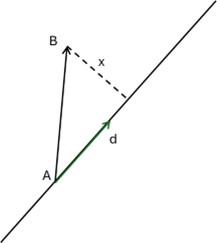
\includegraphics[width=0.3\textwidth]{problema2}\\
 Para encontrar la distancia más corta $x$ entre $B$ y $l$ debemos encontrar un vector formado entre un punto de la recta y $B$, para así proyectarlo sobre la recta y restar el vector encontrado con dicha proyección.
 \par \parskip 8mm
 Observamos gracias a la figura que podemos obtener un vector $u$ a partir de los puntos $A$ y $B$, obteniendo así:
 \begin{equation} \setcounter{equation}{1}
    u=\begin{bmatrix}-2&-1&1\\\end{bmatrix} \nonumber
 \end{equation}\\
 Sabemos que la proyección esta definida como:
 \begin{equation}
    {\rm proy}_du=\frac{u\cdot d}{\left|d\right|^2}d \label{eq:proy}
 \end{equation}\\
 Sustituyendo los vectores $d$ y $u$ en \eqref{eq:proy} tenemos que:
 \begin{gather}
    u\cdot d=\begin{bmatrix}-2&-1&1\\\end{bmatrix}
    \begin{bmatrix}-1\\1\\0\\\end{bmatrix}=1\nonumber\\\nonumber\\
    |d|^2={\sqrt{(-1)^2+(1)^2}}^2=2\nonumber\\\nonumber\\
    {\rm proy}_du=\frac{1}{2} \begin{bmatrix}-1\\1\\0\\\end{bmatrix}=\begin{bmatrix}-\frac{1}{2}\\\frac{1}{2}\\0\\\end{bmatrix}\label{eq:proyr}
 \end{gather}\\
 Ahora para obtener a $x$ tenemos que:
 \begin{equation}
    x=|u-{\rm proy}_du|=\begin{vmatrix}-2+\frac{1}{2},&-1-\frac{1}{2},&1\\\end{vmatrix}=\begin{vmatrix}-\frac{3}{2},&-\frac{3}{2},&1\\\end{vmatrix}\label{eq:distancia}
 \end{equation}\\
 Resolviendo (\ref{eq:distancia}) obtenemos que la distancia entre $B$ y $l$ es:
 \begin{equation}
    x=2.345\ u \nonumber
 \end{equation}
\clearpage
%%%%%%%%PROBLEMA 3%%%%%%%%%%%%
\item Sea la matriz $A$ y suponiendo que $a_{11} a_{22}-a_{12}a_{21}\not= 0$. Demuestre que $A^{-1}=\frac{1}{\left|A\right|}\left[\begin{matrix}a_{22}&-a_{12}\\-a_{21}&a_{11}\\\end{matrix}\right]$.
\par \parskip 8mm
Definiendo a la matriz A como:
\begin{equation} \setcounter{equation}{1}
    A=\left[\begin{matrix}a_{11}&a_{12}\\a_{21}&a_{22}\\\end{matrix}\right]\nonumber
\end{equation}
Debemos tener en cuenta que la determinante de $A$ es:
\begin{equation}
\left|A\right|=a_{11}a_{22}-a_{12}a_{21}\nonumber
\end{equation}
Sabemos que $AA^{-1}=A^{-1}A=I$. Realizando la operación obtenemos que:
\begin{equation}
A^{-1}A=\frac{1}{\left|A\right|}\left[\begin{matrix}a_{22}&-a_{12}\\-a_{21}&a_{11}\\\end{matrix}\right]\left[\begin{matrix}a_{11}&a_{12}\\a_{21}&a_{22}\\\end{matrix}\right]=\frac{1}{\left|A\right|}\left[\begin{matrix}a_{22}a_{11}-a_{12}a_{21}&a_{22}a_{12}-a_{12}a_{22}\\-a_{21}a_{11}+a_{11}a_{21}&-a_{21}a_{12}+a_{11}a_{22}\\\end{matrix}\right]\nonumber
\end{equation}
Podemos percatarnos que los elementos de la diagonal principal son igual a la determinante de la matriz $A$ y los otros dos elementos da igual a cero. Quedando:
\begin{equation}
\frac{1}{\left|A\right|}\left[\begin{matrix}\left|A\right|&0\\0&\left|A\right|\\\end{matrix}\right]=\left[\begin{matrix}1&0\\0&1\\\end{matrix}\right]=I\nonumber
\end{equation}

Quedando demostrado que $A^{-1}$ es la inversa de $A$.

\clearpage
%%%%%%%%%%%%%%PROBLEMA 4%%%%%%%%%%%%%%%%%%%%%
\item 	Sea $P_{1}=(1, 1, -\frac{1}{4})$ y $\overrightarrow{n_{1}}=[3, 3,8]$ un punto conocido en $\pi_{1}$ y un vector normal a este plano, respectivamente. Así como $P_{2}=(1, 1, \frac{11}{6})$ y $\overrightarrow{n_{2}}=[3, 3, -6]$ otro punto en $\pi_{2}$ y un vector normal a este plano. Determine todos los puntos de intersección entre los planos $\pi_{1}$ y $\pi_{2}$.
\par \parskip 8mm
Teniendo en cuenta la forma normal de la ecuación del plano:
\begin{equation} \setcounter{equation}{1}
    \overrightarrow{n}Q=\overrightarrow{n}P \label{eq:normal}
\end{equation}
Siendo $\overrightarrow{n}$ un vector normal al plano, $Q$ y $P$ un punto en el plano. Sustituyendo en \eqref{eq:normal} los puntos y vetores del problema, tenemos que:\\\\
Para $\pi_{1}$:
\begin{equation} 
\left[\begin{matrix}3&3&8\\\end{matrix}\right]\left[\begin{matrix}x\\y\\z\\\end{matrix}\right]=\left[\begin{matrix}3&3&8\\\end{matrix}\right]\left[\begin{matrix}1\\1\\-\frac{1}{4}\\\end{matrix}\right]\label{eq:normal1}
\end{equation}
Para $\pi_2$:
\begin{equation}
\left[\begin{matrix}3&3&-6\\\end{matrix}\right]\left[\begin{matrix}x\\y\\z\\\end{matrix}\right]=\left[\begin{matrix}3&3&-6\\\end{matrix}\right]\left[\begin{matrix}1\\1\\\frac{11}{6}\\\end{matrix}\right]\label{eq:normal2}
\end{equation}
Podemos obtener a partir de \eqref{eq:normal1} y \eqref{eq:normal2} la forma general de la ecuación para $\pi_{1}$ y $\pi_{2}$:
\begin{gather}
3x+3y+8z=4\label{eq:plano1}\\
3x+3y-6z=-5\label{eq:plano2}
\end{gather}
Para determinar todos los puntos de intersección entre los planos debemos resolver este sistema de ecuaciones, usando la eliminación Gauss-Jordan con \eqref{eq:plano1} y \eqref{eq:plano2}, obtenemos que:
\begin{gather}
\left(\begin{matrix}3&3&8\\3&3&-6\\\end{matrix}\middle|\begin{matrix}4\\-5\\\end{matrix}\right)\buildrel R_2=R_2-R_1\over\longrightarrow\left(\begin{matrix}3&3&8\\0&0&-14\\\end{matrix}\middle|\begin{matrix}4\\-9\\\end{matrix}\right){\buildrel R_2=-\frac{R_2}{14}\over\longrightarrow}\left(\begin{matrix}3&3&8\\0&0&1\\\end{matrix}\middle|\begin{matrix}4\\\frac{9}{14}\\\end{matrix}\right)\nonumber\\\nonumber\\
{\buildrel R_1=R_1-8R_2\over\longrightarrow}\left(\begin{matrix}3&3&0\\0&0&1\\\end{matrix}\middle|\begin{matrix}-\frac{8}{7}\\\frac{9}{14}\\\end{matrix}\right){\buildrel R_1=\frac{R_1}{3}\over\longrightarrow}\left(\begin{matrix}1&1&0\\0&0&1\\\end{matrix}\middle|\begin{matrix}-\frac{8}{21}\\\frac{9}{14}\\\end{matrix}\right)\label{eq:puntosint}
\end{gather}\\
Resolviendo la matriz obtenida en \eqref{eq:puntosint}, tenemos como resultado que los puntos de intersección están conformados por:
\begin{equation}
    x=x,\ \ y=x+\frac{8}{21},\ \ z=\frac{9}{14},\ \ -\infty<x<\infty\nonumber
\end{equation}

\clearpage
%%%%%%%%%%%%%%%%%%PROBLEMA 5%%%%%%%%%%%%%%%%%%%%%%%
\item 	Sea $A=\begin{bmatrix}2&6\\8&-6\\\end{bmatrix}$, encuentre un vector no nulo $b=\begin{bmatrix}x\\y\\\end{bmatrix}$ tal que $Ab=6b$.
\par \parskip 8mm
Sustituyendo la matriz $A$ y el vector $b$ en la ecuación $Ab=6b$ tenemos
\begin{equation} \setcounter{equation}{1}
    \left[\begin{matrix}2&6\\8&-6\\\end{matrix}\right]\left[\begin{matrix}x\\y\\\end{matrix}\right]=6\left[\begin{matrix}x\\y\\\end{matrix}\right]\nonumber
\end{equation}
Teniendo así el sistema de ecuaciones:
\begin{gather}
    2x+6y=6x\nonumber\\
    8x-6y=6y\nonumber 
\end{gather}
Resolviendo el sistema de ecuaciones obtenemos que:
\begin{equation} 
    y=\frac{2}{3}x\label{eq:resultadov}
\end{equation}
Por lo que, sustituyendo a \eqref{eq:resultadov} en el vector $b$, obtenemos el vector:
\begin{equation}
    b=\left[\begin{matrix}x\\\frac{2}{3}x\\\end{matrix}\right],\ \ para\ x\not=0 \nonumber
\end{equation}
Para $x=1$ tenemos que:
\begin{equation} \setcounter{equation}{1}
    b=\left[\begin{matrix}1\\\frac{2}{3}\\\end{matrix}\right]\nonumber
\end{equation}
Obteniendo asi un vector no nulo $b$.


\clearpage
%%%%%%%%%%%%%%%%%%PROBLEMA 6%%%%%%%%%%%%%%%%%%%%
\item 	Determine si la matriz $A=\begin{bmatrix}2&3&2&4\\4&10&-4&0\\-3&-2&-5&-2\\-2&4&4&-7\\\end{bmatrix}$ es invertible. Pista factorización $LU$.
\par \parskip 8mm
Si $A$ es una matriz singular (no invertible) entonces la forma escalonada por renglones de $A$ debe tener al menos un renglón de ceros al igual que la forma triangular de $A$, lo que implica que la factorización $LU$ no sería única. Por la definición de la factorización $LU$:
\begin{equation} 
    \left[\begin{matrix}2&3&2&4\\4&10&-4&0\\-3&-2&-5&-2\\-2&4&4&-7\\\end{matrix}\right]=\begin{bmatrix}1&0&0&0\\a&1&0&0\\b&c&1&0\\d&e&f&1\\\end{bmatrix}\begin{bmatrix}2&3&2&4\\0&u&v&w\\0&0&x&y\\0&0&0&z\\\end{bmatrix}\label{eq:factLU}
\end{equation}
Desarrollando la multiplicacion de matrices en \eqref{eq:factLU} obtenemos la siguiente matriz:
\begin{equation}
    \left[\begin{matrix}2&3&2&4\\2a&3a+u&2a+v&4a+w\\2b&3b+cu&2b+cv+x&4b+cw+y\\2d&3d+eu&2d+ev+fx&4d+ew+fy+z\\\end{matrix}\right]\label{eq:factLU2}
\end{equation}
Resolvemos para encontrar las incógnitas resultando en:
\begin{equation}
    \begin{matrix}a=2&&b=-\frac{3}{2}&&c=\frac{5}{8}&&d=-1\\\\e=\frac{7}{4}&&f=\frac{20}{3}&&u=4&&v=-8\\\\w=-8&&x=3&&y=9&&z=-49\end{matrix}\label{eq:resultadoLU}
\end{equation}
Sustituyendo a \eqref{eq:resultadoLU} en \eqref{eq:factLU} obtenemos así la matriz $L$ y $U$ como:
\begin{equation}
    L=\left[\begin{matrix}1&0&0&0\\2&1&0&0\\-\frac{3}{2}&\frac{5}{8}&1&0\\-1&\frac{7}{4}&\frac{20}{3}&1\\\end{matrix}\right],\ \ U=\left[\begin{matrix}2&3&2&4\\0&4&-8&-8\\0&0&3&9\\0&0&0&-49\\\end{matrix}\right]\nonumber
\end{equation}
Al existir una factorización $LU$ única podemos concluir que la matriz $A$ es invertible.

\clearpage
%%%%%%%%%%%%%%%%%%%%%%%%PROBLEMA 7%%%%%%%%%%%%%%%%%%%%%%%%%%
\item 	Muestre que si $A$ es triangular, entonces el determinante de $A\not=0$, si y solo si todos los elementos en la diagonal son diferentes de cero.
\par \parskip 8mm
Definimos las matrices triangulares $A$ y $B$ como:
\begin{equation} \setcounter{equation}{1}
    A=\left[\begin{matrix}a_{11}&0&0&\cdots&0\\a_{21}&a_{22}&0&\cdots&0\\a_{31}&a_{32}&a_{33}&\cdots&0\\\vdots&\vdots&\vdots&\ddots&\vdots\\a_{n1}&a_{n2}&a_{n3}&\cdots&a_{nn}\\\end{matrix}\right],\ \ B=\left[\begin{matrix}a_{11}&a_{12}&a_{13}&\cdots&a_{1n}\\0&a_{22}&a_{23}&\cdots&a_{2n}\\0&0&a_{33}&\cdots&a_{3n}\\\vdots&\vdots&\vdots&\ddots&\vdots\\0&0&0&\cdots&a_{nn}\\\end{matrix}\right]\nonumber
\end{equation}
Ahora obtendremos las determinantes de dichas matrices:
\begin{gather}
     \left|A\right|=\left|\begin{matrix}a_{11}&0&0&\cdots&0\\a_{21}&a_{22}&0&\cdots&0\\a_{31}&a_{32}&a_{33}&\cdots&0\\\vdots&\vdots&\vdots&\ddots&\vdots\\a_{n1}&a_{n2}&a_{n3}&\cdots&a_{nn}\\\end{matrix}\right|=a_{11}\left|\begin{matrix}a_{22}&0&\cdots&0\\a_{32}&a_{33}&\cdots&0\\\vdots&\vdots&\ddots&\vdots\\a_{n2}&a_{n3}&\cdots&a_{nn}\\\end{matrix}\right|\nonumber\\\nonumber\\
     -0\left|\begin{matrix}a_{21}&0&\cdots&0\\a_{31}&a_{33}&\cdots&0\\\vdots&\vdots&\ddots&\vdots\\a_{n1}&a_{n3}&\cdots&a_{nn}\\\end{matrix}\right|+\ldots=\prod_{n=1}^{\infty}a_{nn}\nonumber  
\end{gather}
\begin{gather}
    \left|B\right|=\left|\begin{matrix}a_{11}&a_{12}&a_{13}&\cdots&a_{1n}\\0&a_{22}&a_{23}&\cdots&a_{2n}\\0&0&a_{33}&\cdots&a_{3n}\\\vdots&\vdots&\vdots&\ddots&\vdots\\0&0&0&\cdots&a_{nn}\\\end{matrix}\right|=a_{11}\left|\begin{matrix}a_{22}&a_{23}&\cdots&a_{2n}\\0&a_{33}&\cdots&a_{3n}\\\vdots&\vdots&\ddots&\vdots\\0&0&\cdots&a_{nn}\\\end{matrix}\right|\nonumber\\
    -a_{12}\left|\begin{matrix}0&a_{23}&\cdots&a_{2n}\\0&a_{33}&\cdots&a_{3n}\\\vdots&\vdots&\ddots&\vdots\\0&0&\cdots&a_{nn}\\\end{matrix}\right|+\ldots=\prod_{n=1}^{\infty}a_{nn}\nonumber
\end{gather}
Podemos observar que para el caso de $|A|$ los elementos de la fila 1 se vuelven cero al descomponerla por cofactores y sucederá lo mismo a la hora de calcular la determinante del cofactor $A_{11}$. Para el caso de $|B|$ podemos observar que para los cofactores distintos de $A_{11}$ son igual a cero debido a que siempre contendrán su primera columna llena de ceros y sucede algo similar al caso de $|A|$ con el determinante del cofactor $A_{11}$. Con esto en mente podemos concluir que, para las matrices triangulares, su determinante se calcula como el producto de los elementos de su diagonal principal.

\end{enumerate}

\end{document}